\documentclass{beamer}
\usepackage[utf8]{inputenc}
\usepackage{lipsum}
\usepackage{multirow}
\usepackage{graphicx}
\graphicspath{ {./images/} }
\usepackage{cellspace}
\setlength\cellspacetoplimit{5pt}
\setlength\cellspacebottomlimit{5pt}

\usetheme{Madrid}
\usecolortheme{default}
%Information to be included in the title page:
\title{Analysis of Electricity Consumption in India}
\author{Group- WATTSUP}

\date{November 2021}

\begin{document}
\AtBeginSection[]{
  \begin{frame}{Outline}
  \small \tableofcontents[currentsection, hideothersubsections]
  \end{frame} 
}

\frame{\titlepage}
\begin{frame}
\frametitle{Table of Contents}
\tableofcontents
\end{frame}


\section{Group Members- WATTSUP}
\begin{frame}
\frametitle{Group Members- WATTSUP}
\centering
\begin{tabular}{|Sc|Sl|Sl|Sl|}

\hline
    Ser & Name &  Reg number & Background \\ 
\hline 
    1 & Karan Chawla & EPABABL0523016 & \parbox{3 cm}{Director, MIS \& Analytics,\\ American Express} \\ 
\hline
    2 & Krishna Kumar & EPABABL0523017 & \parbox{3 cm}{Manager, \\Niva Bupa Health Insurance}\\ 

    \hline
    3 & Roopesh Kesav & EPABABL0523032 & Indian Navy\\ 
\hline
\end{tabular}
\end{frame}
\section{Problem Statement}
\begin{frame}{Problem Statement}
    \begin{block}{Remark}
    \parbox{\linewidth}{
    Understanding energy consumption patterns, sources, and trends for sustainable development, energy planning, and environmental management.
    }
    \end{block}
    
\end{frame}
\section{Goals}
\begin{frame}{Goals}
    \begin{itemize}
        \item \textbf{\underline{Data Collection}}. Historical data on electrical energy consumption,production, and related factors for different states and sectors.
        \begin{itemize}
            \item indiastat.com - under power category.
        \end{itemize}
        \pause
        \item \textbf{\underline{Data Preprocessing}}. Handle missing values, outliers, and inconsistencies.
        \begin{itemize}
            \item Inconsistencies - between years.
            \item Creation of states/regions over time.
            \item Inconsistency in data available - column /rows splits
        \end{itemize}
        
        
        
    \end{itemize}
\end{frame}
\begin{frame}{Goals}
    \begin{itemize}
        \item \textbf{\underline{Descriptive Analysis}}. Visualizing trends, variations, and patterns in energy consumption across regions and sectors.
        \pause
        \item \textbf{\underline{Temporal Analysis}}. Consumption  over time considering
        \begin{itemize}
            \item Population growth.
            \item Economic development.
            \item Technological advancements.
        \end{itemize}
        \pause
        \item \textbf{\underline{Spatial Analysis}}.Regional Disparities in energy consumption.
        \pause
        \item \textbf{\underline{Source Analysis}}.Analyse shift in energy source and its implications.
        \pause
        \item \textbf{\underline{Sectoral Analysis}.}Energy consumption by sectors.
        
        
    \end{itemize}
\end{frame}

\section{Status - as on date}
\begin{frame}{Present Status- Data Collection and Preprocessing}

    
    \centering
    \resizebox{\textwidth}{!}{%
    \begin{tabular}{|c|l|l|l|}

    \hline
        Ser & Data Description &  Duration & Status \\ 
    \hline
        1 & Electricity Consumers  & 2008-2021 & \multirow{8}{*} {\parbox{5cm}{Data Downloaded. \\Preprocessing in progress.
}}\\ 
    \cline{1-3}
        2 & Electricity Tariff and Duty - & 2011,2015,2021 & \\ 
    \cline{1-3}
        3 & Electrification  & 2002-2022 & \\ 
    \cline{1-3}
        4 & Power Allocation  & 2010-2019 & \\ 
    \cline{1-3}
        5 & Power Connected Load   & 2010-2021 & \\ 
    \cline{1-3}
        6 & Power Consumption and Sale  & 2011-2022 & \\ 
    \cline{1-3}
    7 & Power Generation   & 2014-2023 & \\ 
    \cline{1-3}
    8 & 
Transmission and Distribution  & 2013-2022 & \\ 
    \hline
    \end{tabular}
    }
    \end{frame}

\begin{frame}{Consumers Data - snapshot from indiastat}
    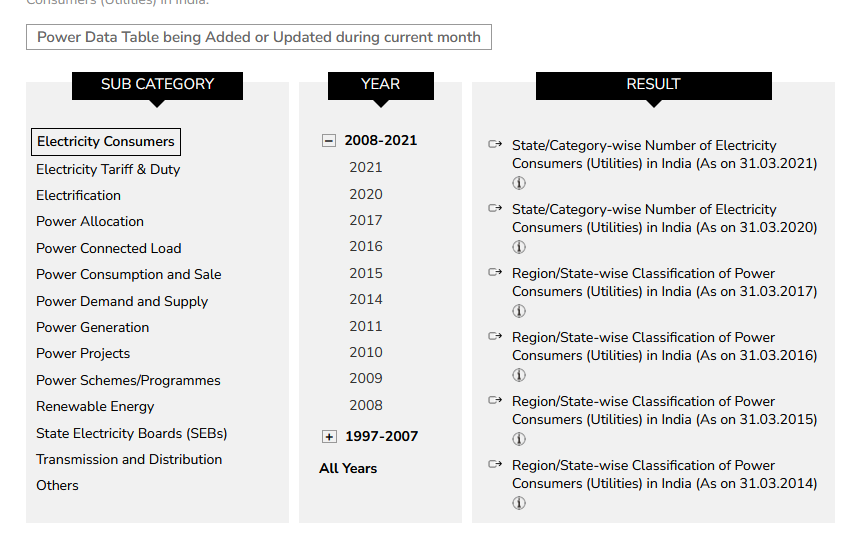
\includegraphics[width = \textwidth]{images/indiastat-1.png}
\end{frame}

\begin{frame}{Consumers Data - Preprocess and Visualisation}
    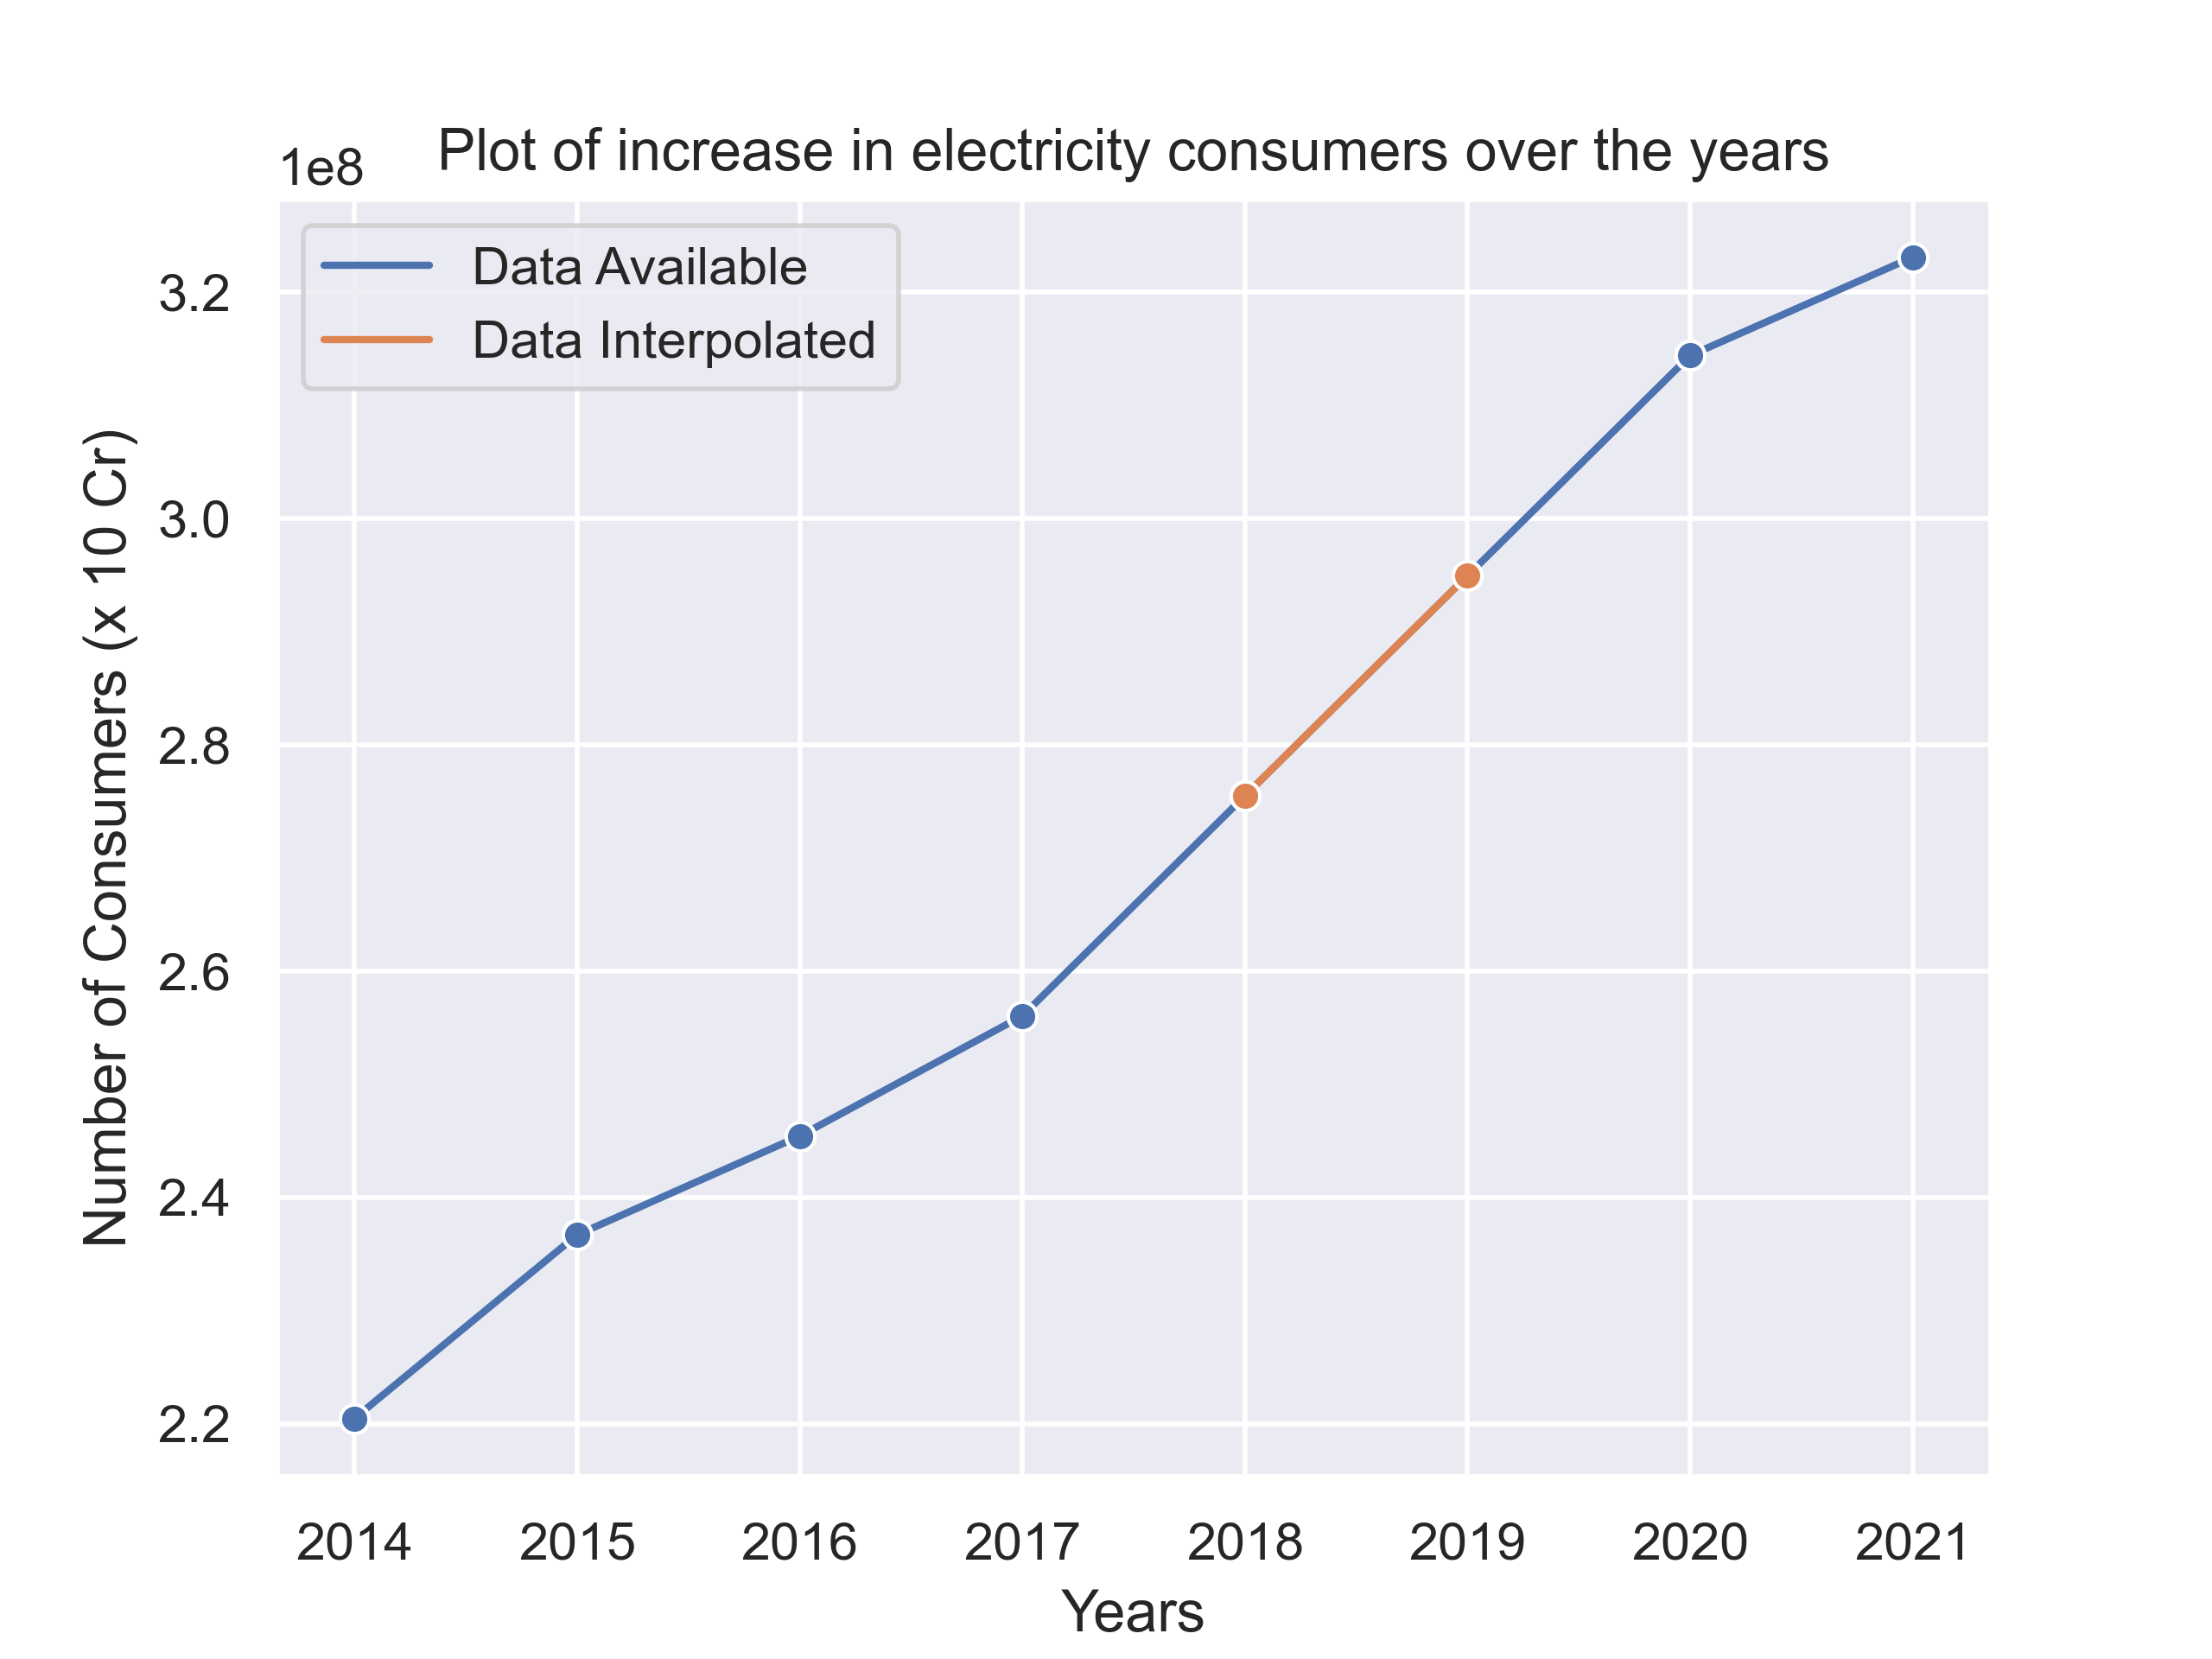
\includegraphics[scale=.6]{images/Cons.png}
\end{frame}

\begin{frame}{Consumers Data - Preprocess and Visualisation}
    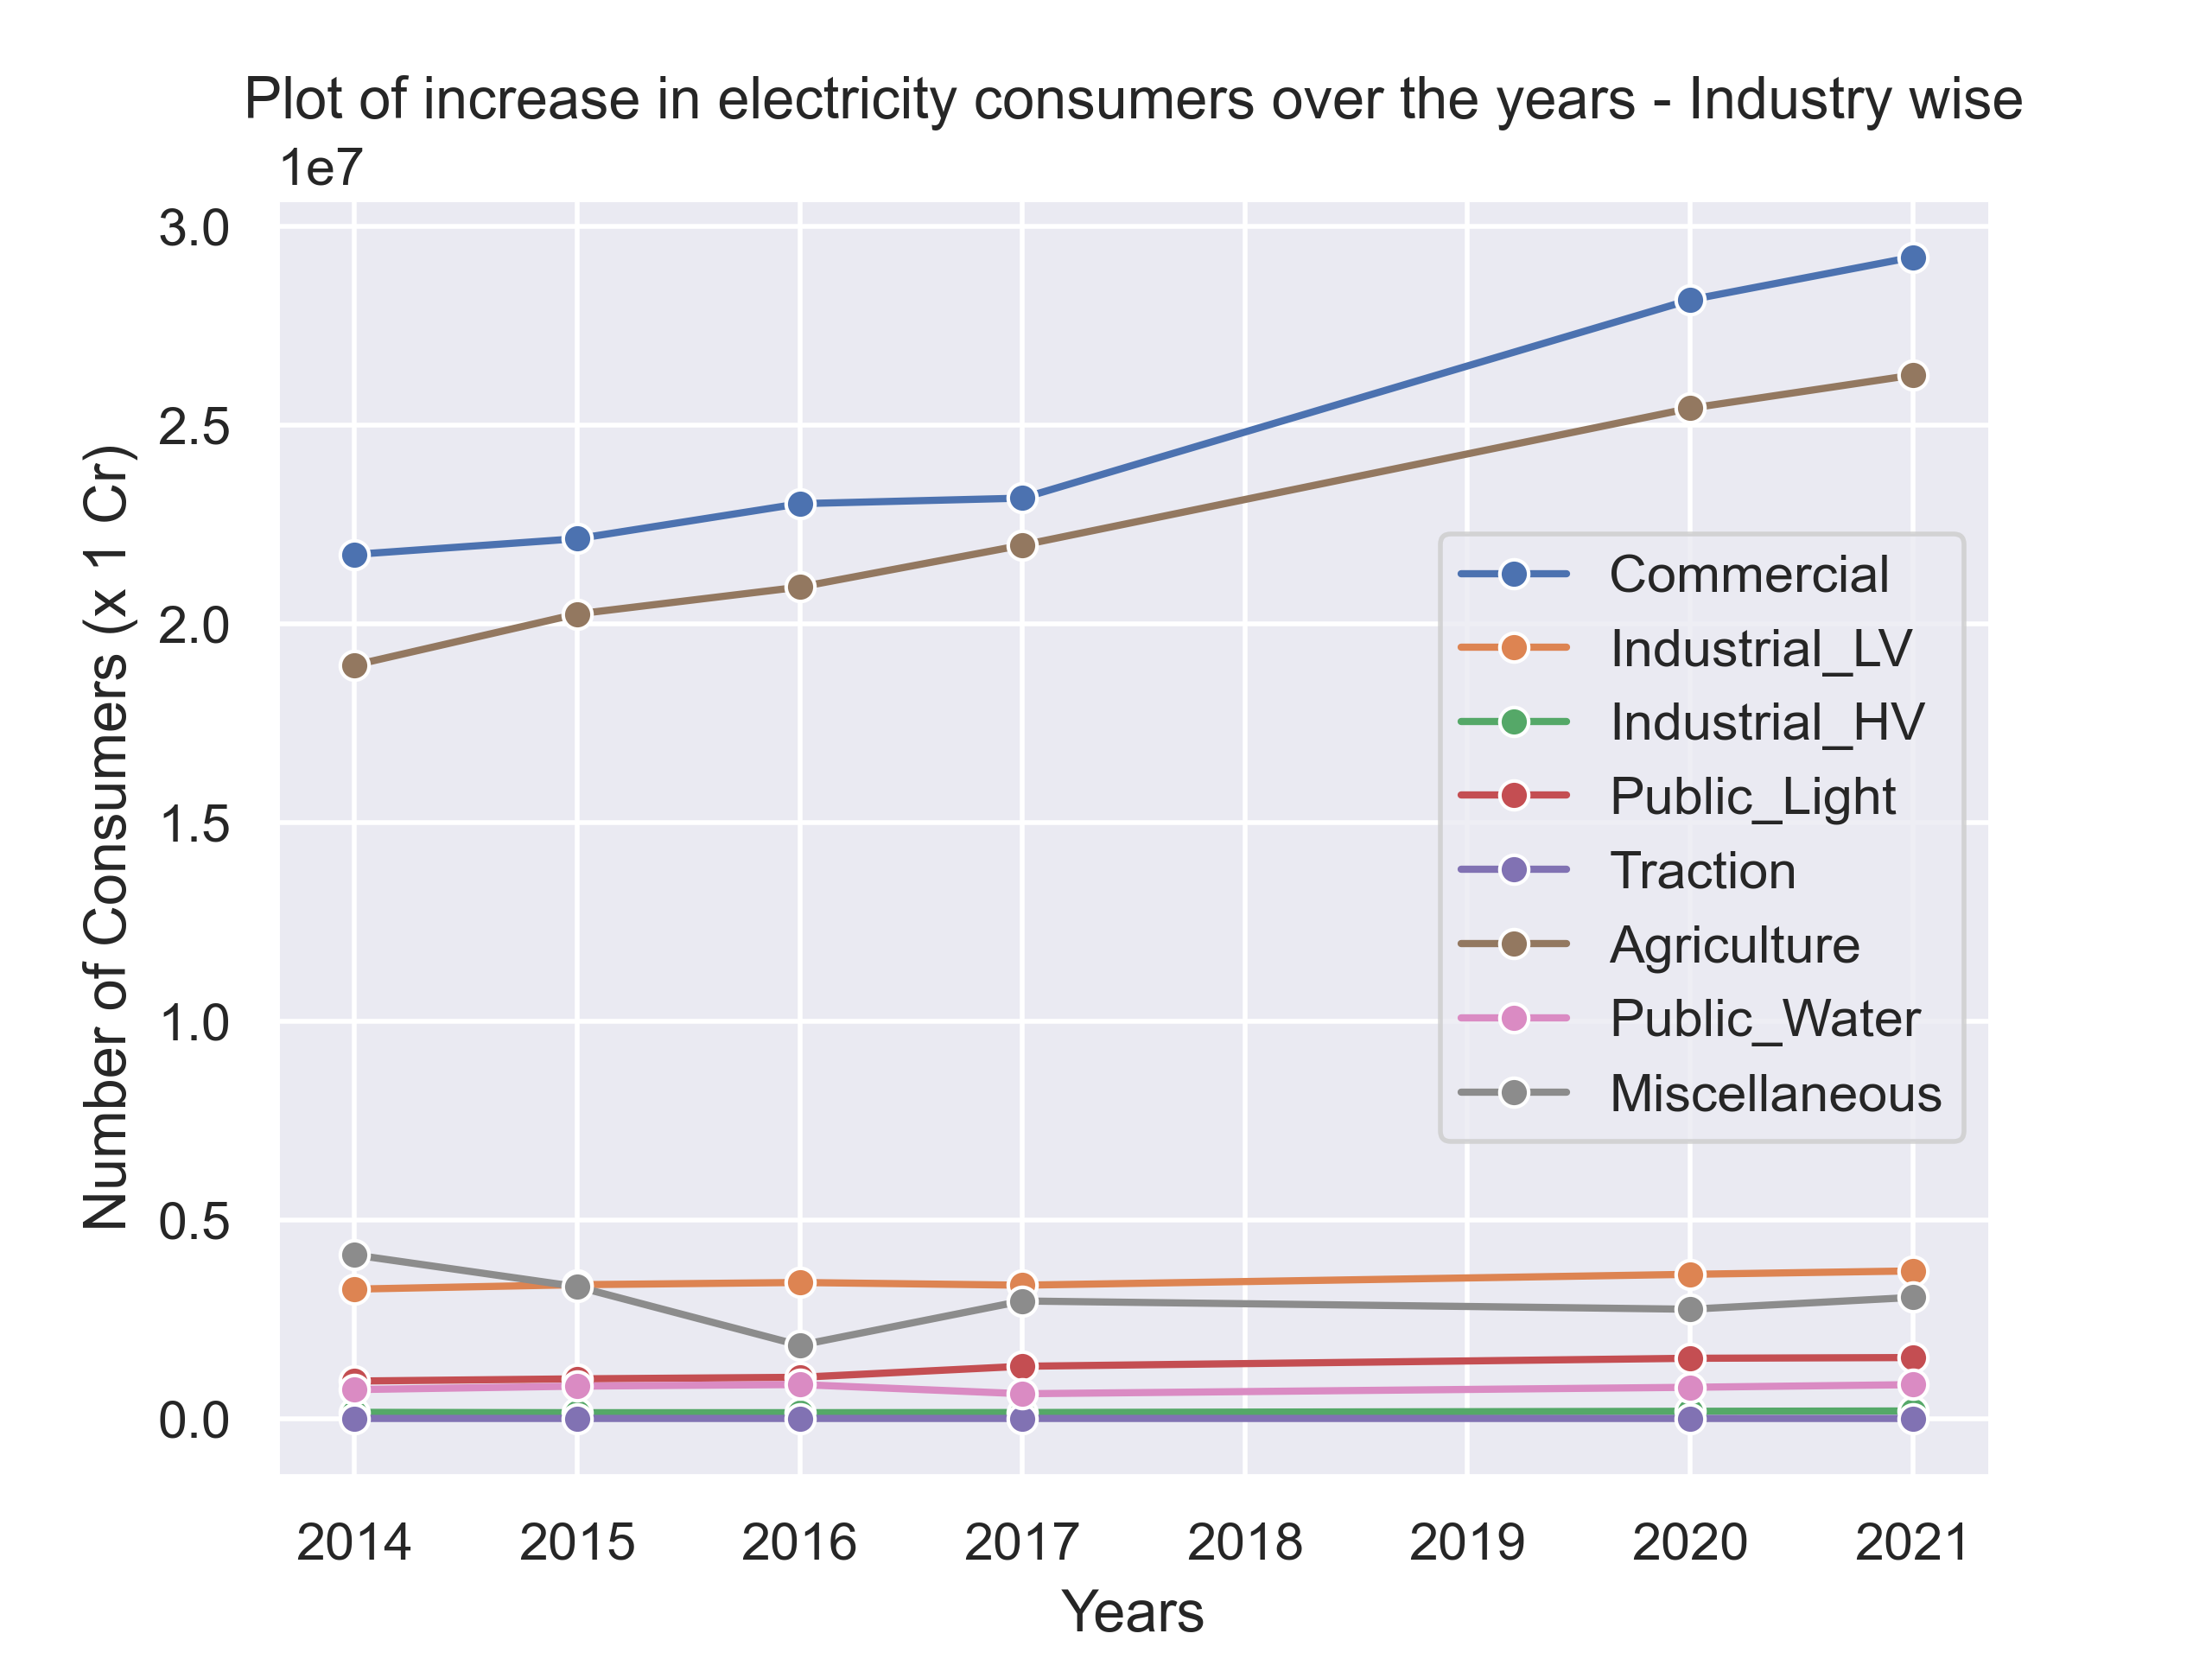
\includegraphics[scale=.6]{images/Cons_Ind.png}
\end{frame}

\section{Doubts, Clarification, Queries}
\begin{frame}{Doubts, Clarification, Queries}
    \begin{itemize}
        \item R or Python
        \item Scope of the Project
        
    \end{itemize}
    
\end{frame}
\end{document}
